\clearpage\begin{figure}[p]\centering
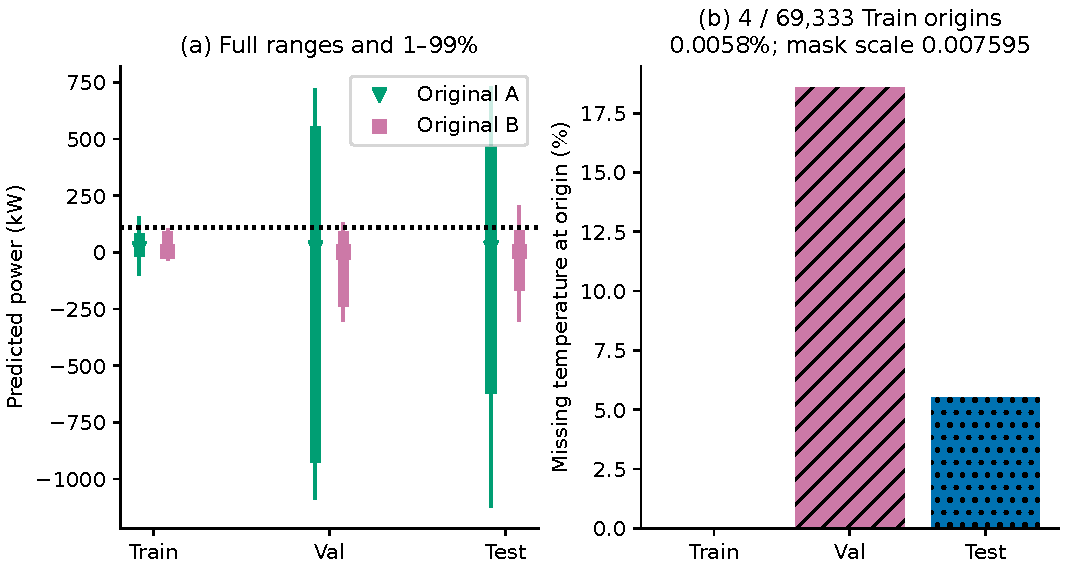
\includegraphics[width=0.98\textwidth,height=0.86\textheight,keepaspectratio]{fixed_period_figures/figS11_yulara_diagnostic.pdf}
\caption{Yulara original Ridge distributions and weather-missing exposure: 4/69333 Train origins (0.0058\%). Thin lines show extrema, thick lines 1st–99th percentiles, markers medians. The dotted line is the Train target maximum, not a clipping threshold.}
\label{figs:figS11_yulara_diagnostic}
\end{figure}
\clearpage\begin{figure}[p]\centering
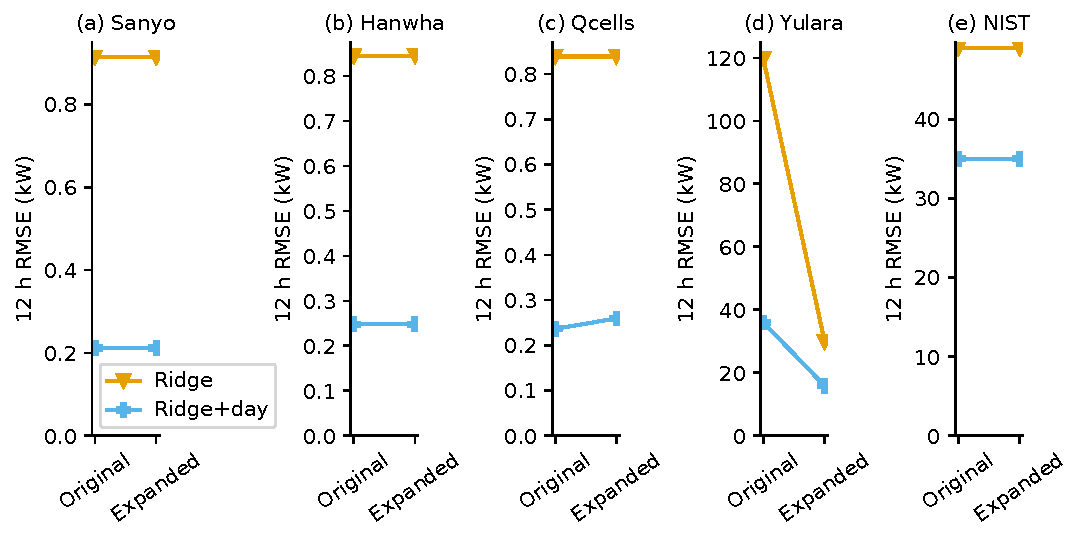
\includegraphics[width=0.98\textwidth,height=0.86\textheight,keepaspectratio]{fixed_period_figures/figS12_alpha_sensitivity.pdf}
\caption{Uniform expanded alpha grid $10^{-4}$ through $10^8$, selected solely by full-H144 Validation MSE for all five systems and both information sets. Original and expanded Test errors use identical Daily-matched full targets; all ten comparisons are shown.}
\label{figs:figS12_alpha_sensitivity}
\end{figure}
\clearpage\begin{figure}[p]\centering
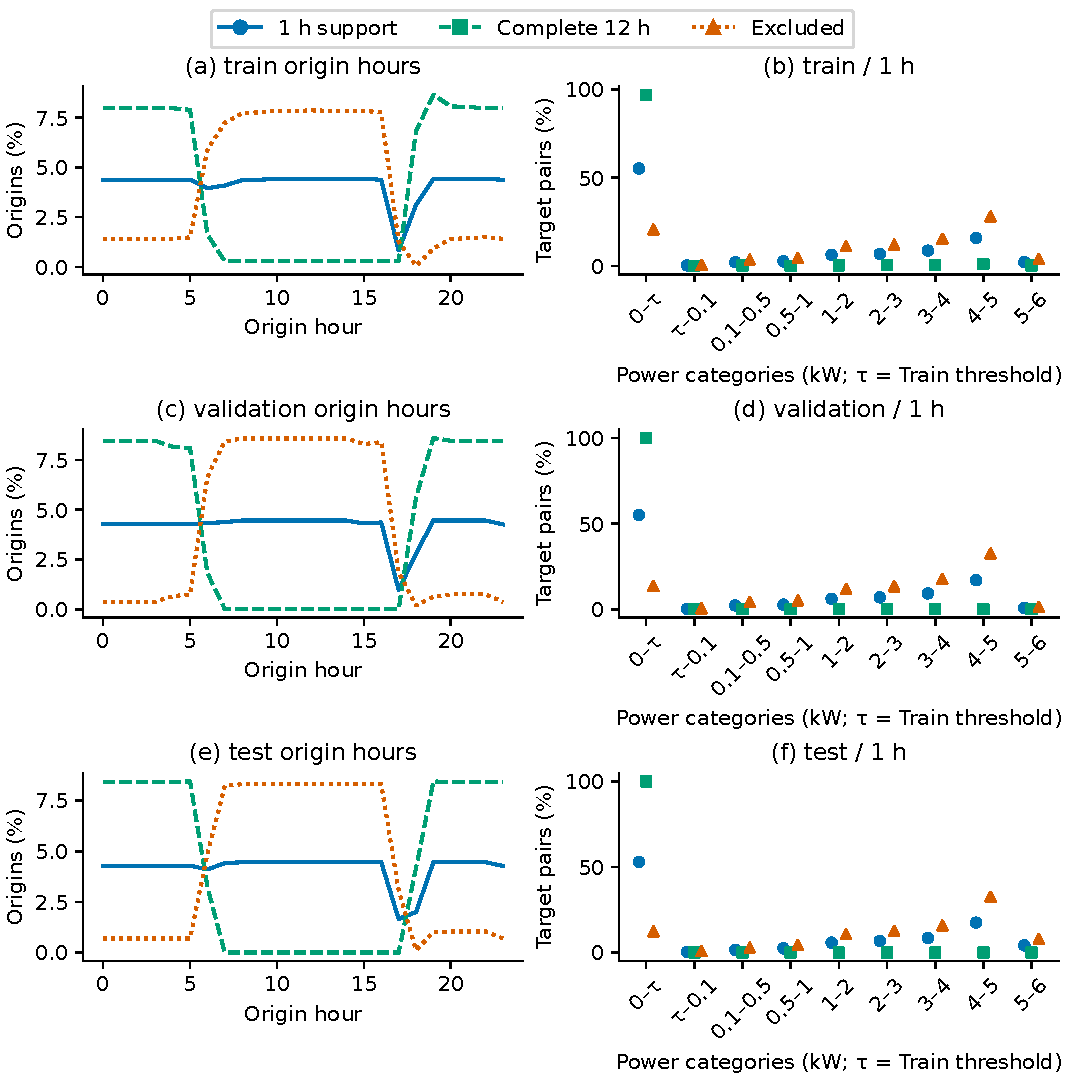
\includegraphics[width=0.98\textwidth,height=0.86\textheight,keepaspectratio]{fixed_period_figures/figS10_qcells_support.pdf}
\caption{Qcells support composition in every split. Left: origin-hour proportions. Right: categorical points for unequal-width power bins, normalized by pairs in the displayed bins. Complete-H144 conditioning selects different hours and power ranges in Train and Validation as well as Test.}
\label{figs:figS10_qcells_support}
\end{figure}
\clearpage\begin{figure}[p]\centering
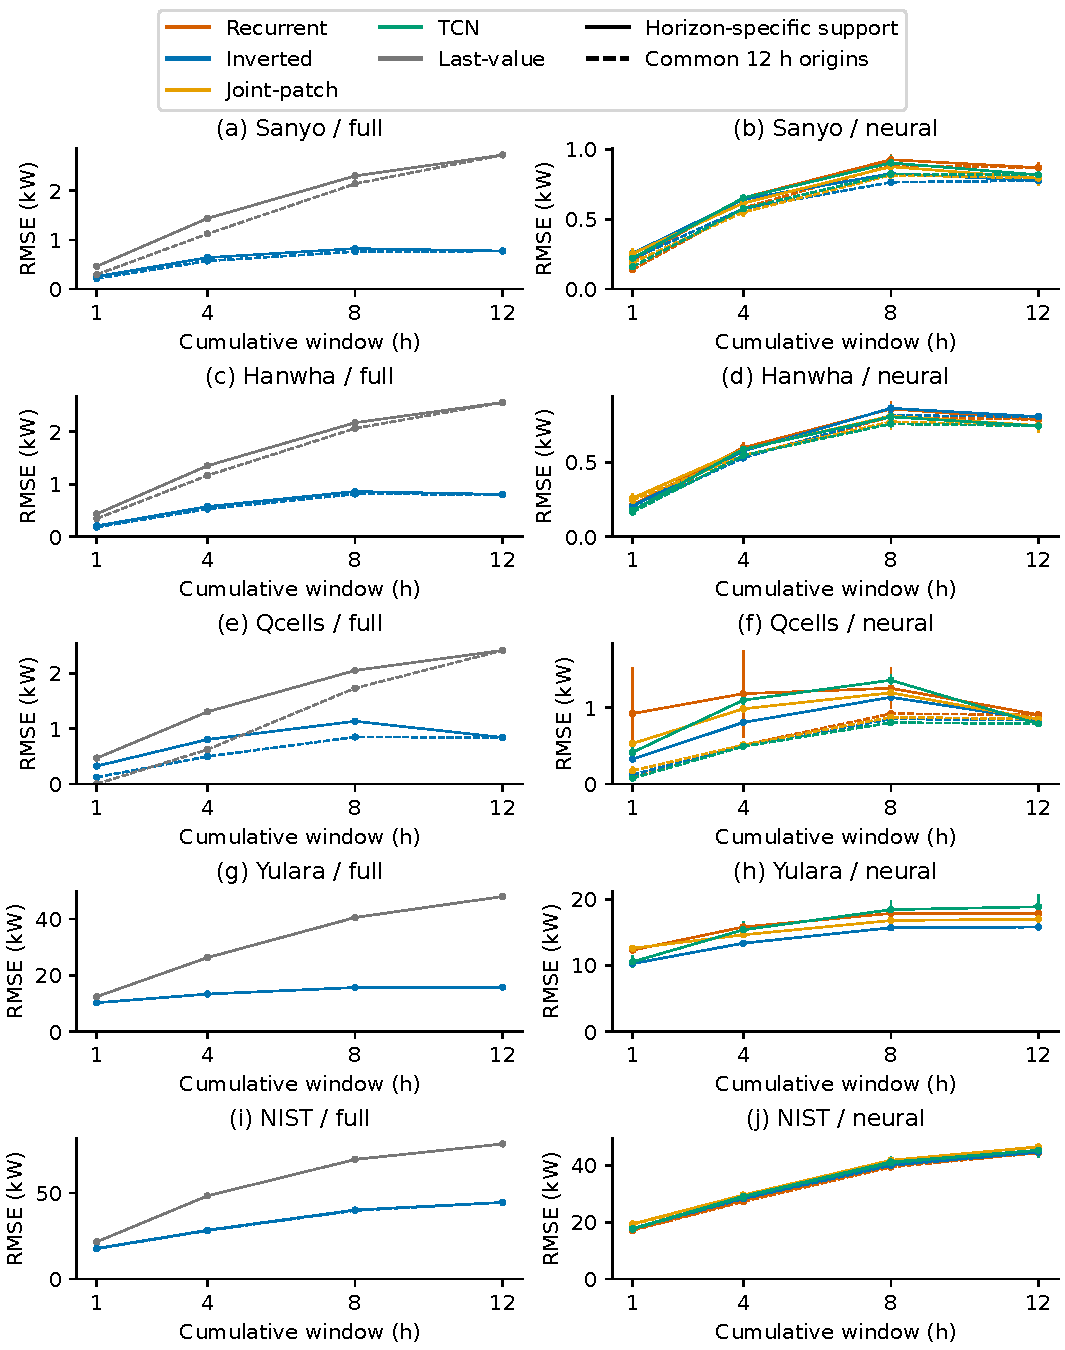
\includegraphics[width=0.98\textwidth,height=0.86\textheight,keepaspectratio]{fixed_period_figures/figS2_common_origins.pdf}
\caption{Horizon-specific support (solid) versus common complete-twelve-hour origins (dashed) cumulative errors. Bars are seed SD. Left panels preserve reference error ranges; right panels show neural detail on separately labelled axes.}
\label{figs:figS2_common_origins}
\end{figure}
\clearpage\begin{figure}[p]\centering
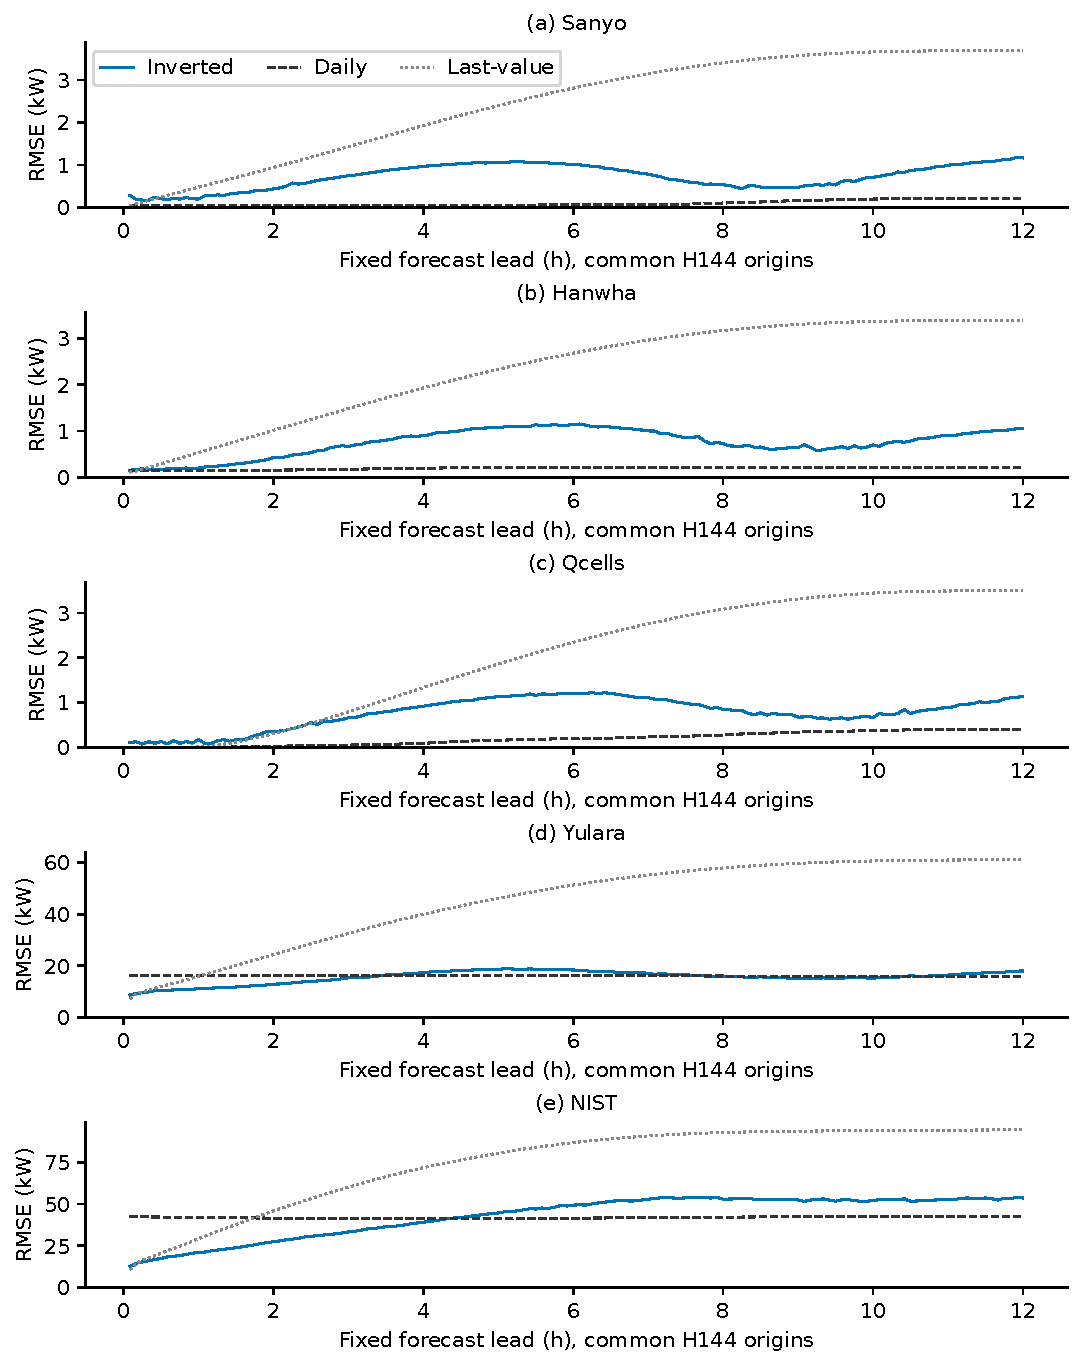
\includegraphics[width=0.98\textwidth,height=0.86\textheight,keepaspectratio]{fixed_period_figures/figS4_fixed_leads.pdf}
\caption{Lead-specific error at each five-minute lead on common complete-H144 origins and Daily-valid targets. These are not cumulative-prefix metrics. Neural curves average per-seed RMSE.}
\label{figs:figS4_fixed_leads}
\end{figure}
\clearpage\begin{figure}[p]\centering
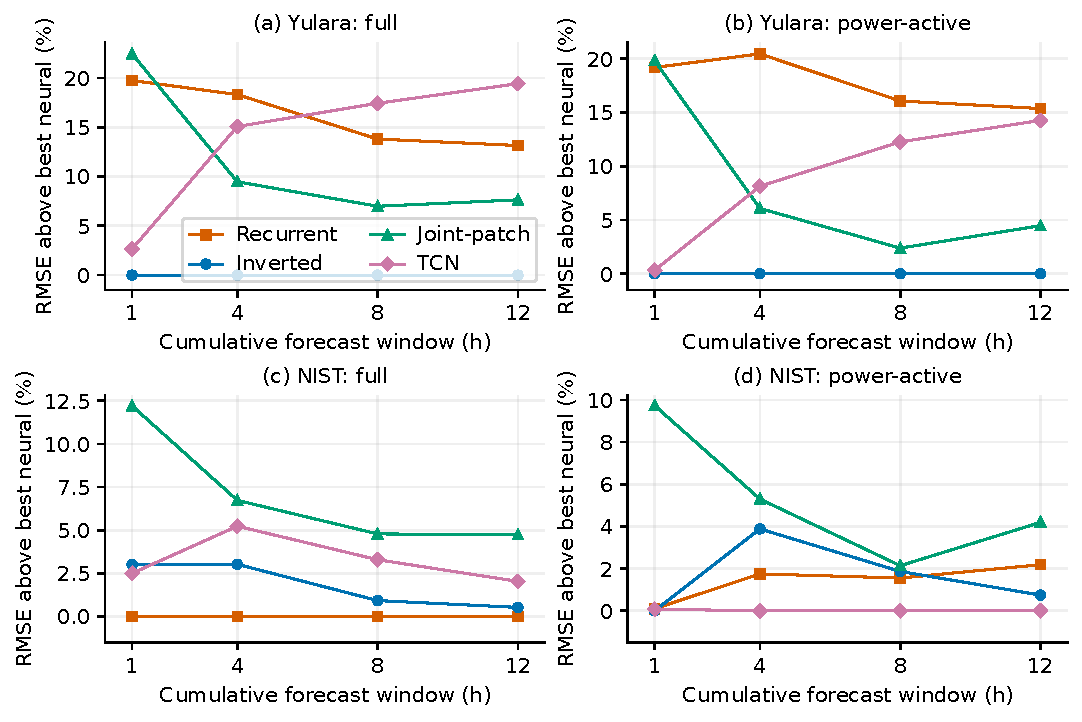
\includegraphics[width=0.98\textwidth,height=0.86\textheight,keepaspectratio]{fixed_period_figures/fig4_neural_gaps.pdf}
\caption{Relative RMSE gaps from the best mean neural implementation in each cumulative window and power scope. Zero identifies the lowest error; small gaps are shown as small gaps rather than enlarged rank differences.}
\label{figs:fig4_neural_gaps}
\end{figure}
\clearpage\begin{figure}[p]\centering
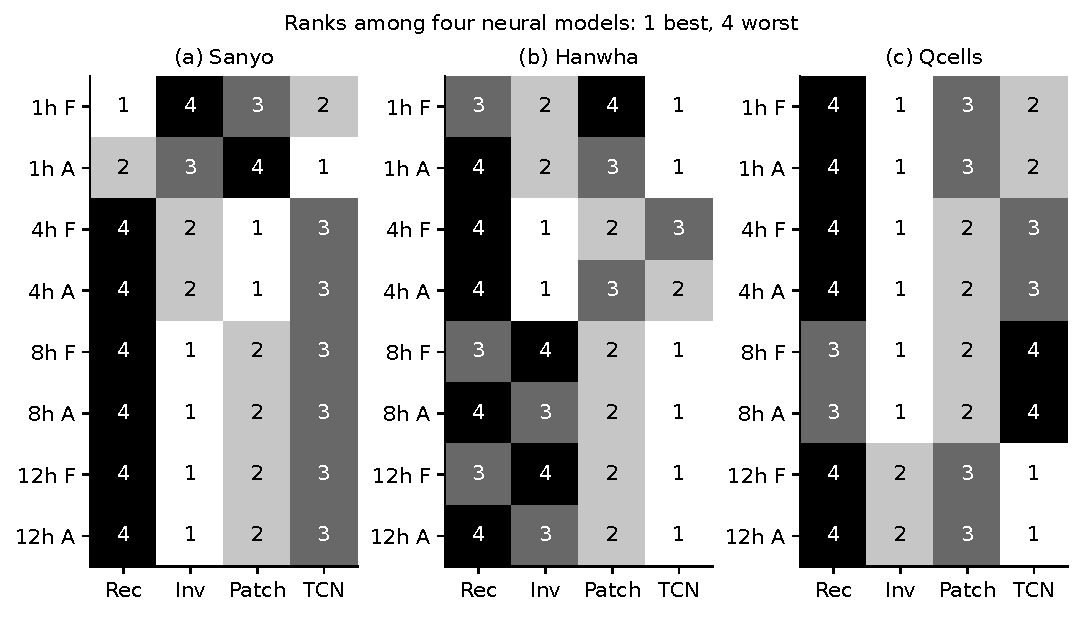
\includegraphics[width=0.98\textwidth,height=0.86\textheight,keepaspectratio]{fixed_period_figures/figS1_alice_ranks.pdf}
\caption{Alice neural ranks by cumulative window and target-power scope. F: full; A: power-active; four discrete rank levels.}
\label{figs:figS1_alice_ranks}
\end{figure}
\clearpage\begin{figure}[p]\centering
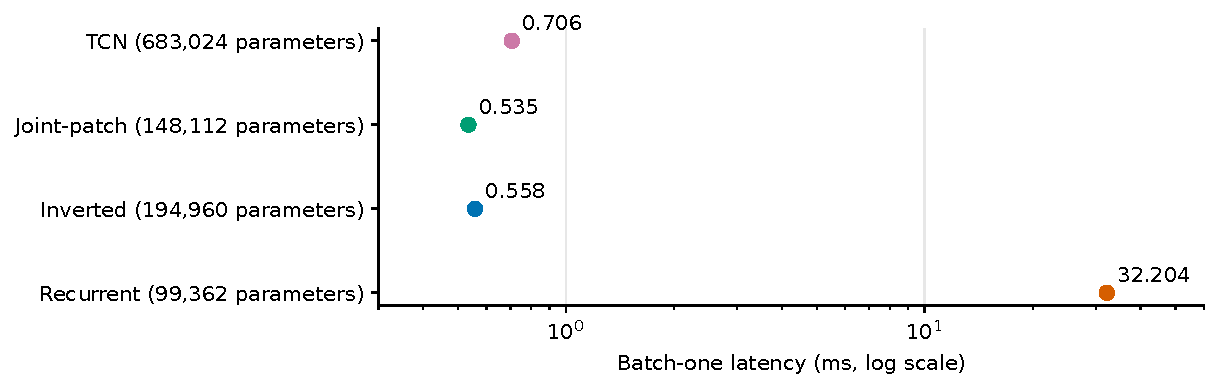
\includegraphics[width=0.98\textwidth,height=0.86\textheight,keepaspectratio]{fixed_period_figures/figS3_latency.pdf}
\caption{Historical 17-channel inference timings on RTX 3060 Laptop GPU, excluding loading/preprocessing. Point summaries do not establish a stable difference between 0.535 and 0.558 ms; no new timing experiment.}
\label{figs:figS3_latency}
\end{figure}
\clearpage\begin{figure}[p]\centering
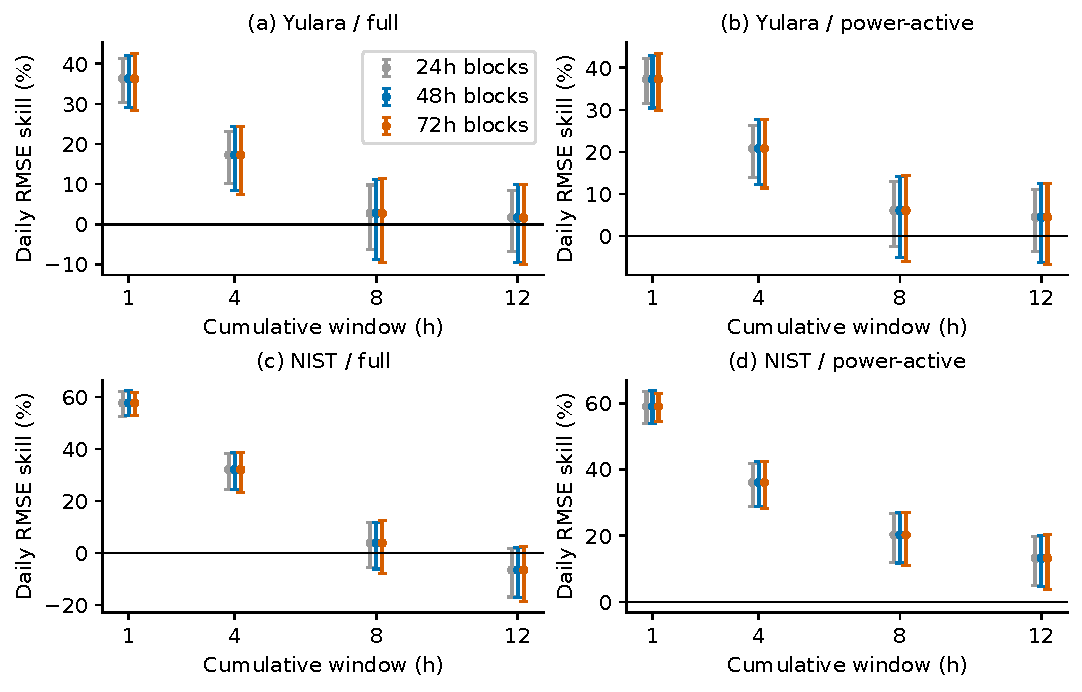
\includegraphics[width=0.98\textwidth,height=0.86\textheight,keepaspectratio]{fixed_period_figures/figS5_block_intervals.pdf}
\caption{Paired temporal-block percentile intervals (2000 resamples; 24/48/72 h). SSE/count is aggregated before each seed RMSE, then seed skills are averaged. These intervals are conditional on observed dates and fitted models, not prediction intervals.}
\label{figs:figS5_block_intervals}
\end{figure}
\clearpage\begin{figure}[p]\centering
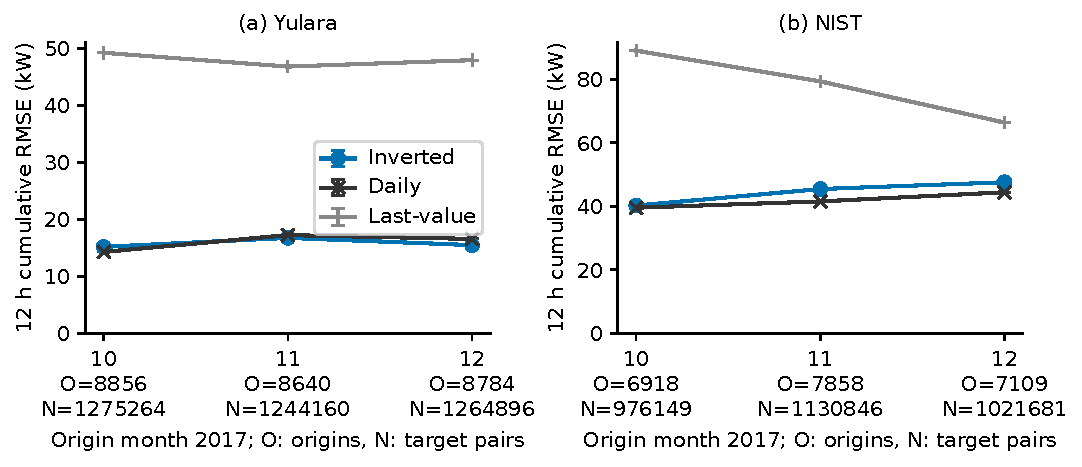
\includegraphics[width=0.98\textwidth,height=0.86\textheight,keepaspectratio]{fixed_period_figures/figS6_monthly.pdf}
\caption{Monthly errors assign each full twelve-hour trajectory to its forecast-origin month on common H144 Daily-valid support. Bars show seed SD. O denotes origins and N scored origin--lead target pairs, printed for each month.}
\label{figs:figS6_monthly}
\end{figure}
\clearpage\begin{figure}[p]\centering
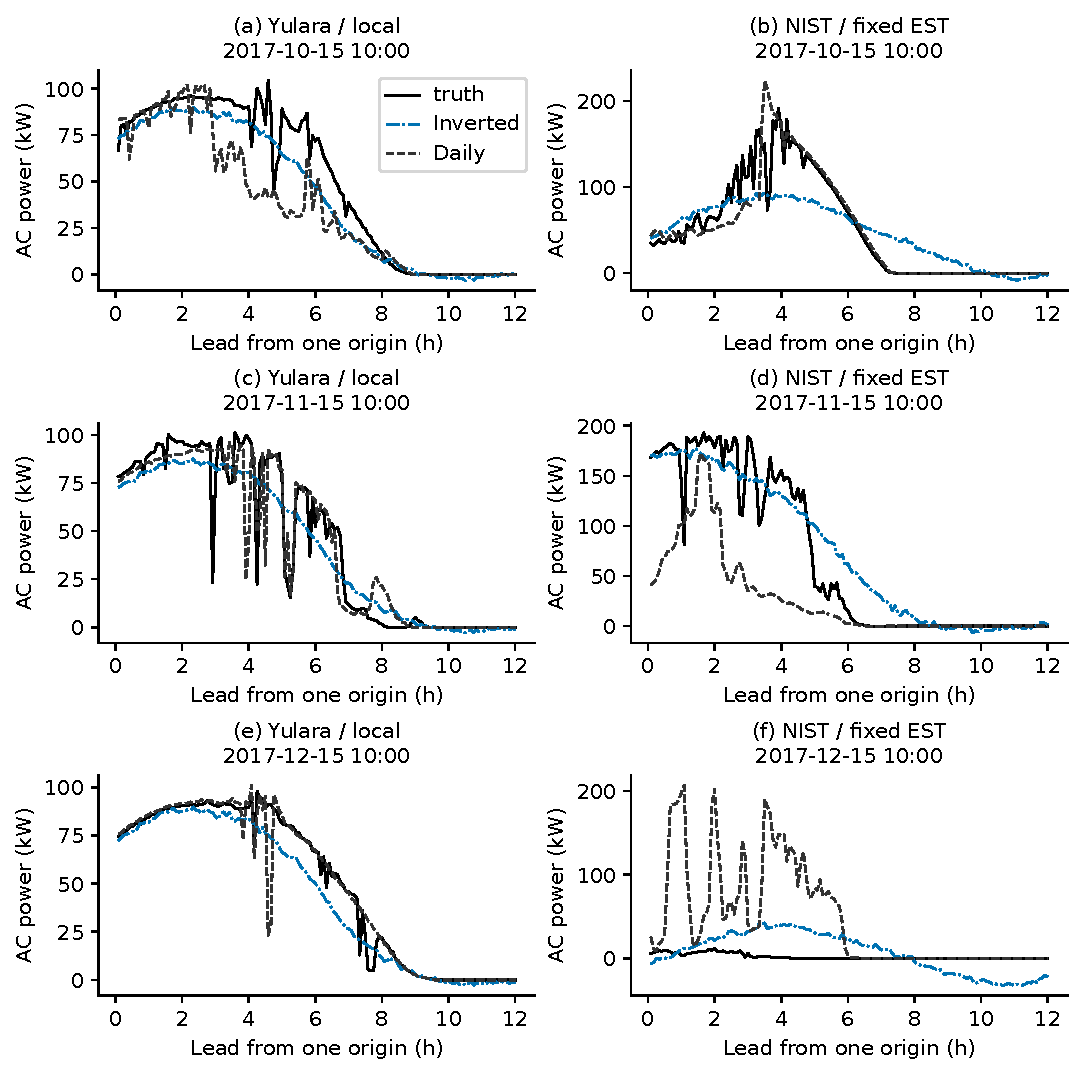
\includegraphics[width=0.98\textwidth,height=0.86\textheight,keepaspectratio]{fixed_period_figures/figS7_cases_fixed.pdf}
\caption{Fixed calendar seed42 trajectories. Fixed cases use the first eligible origin on or after each month’s 15th at 10:00; extremes use original Daily SSE differences and are not representative frequencies.}
\label{figs:figS7_cases_fixed}
\end{figure}
\clearpage\begin{figure}[p]\centering
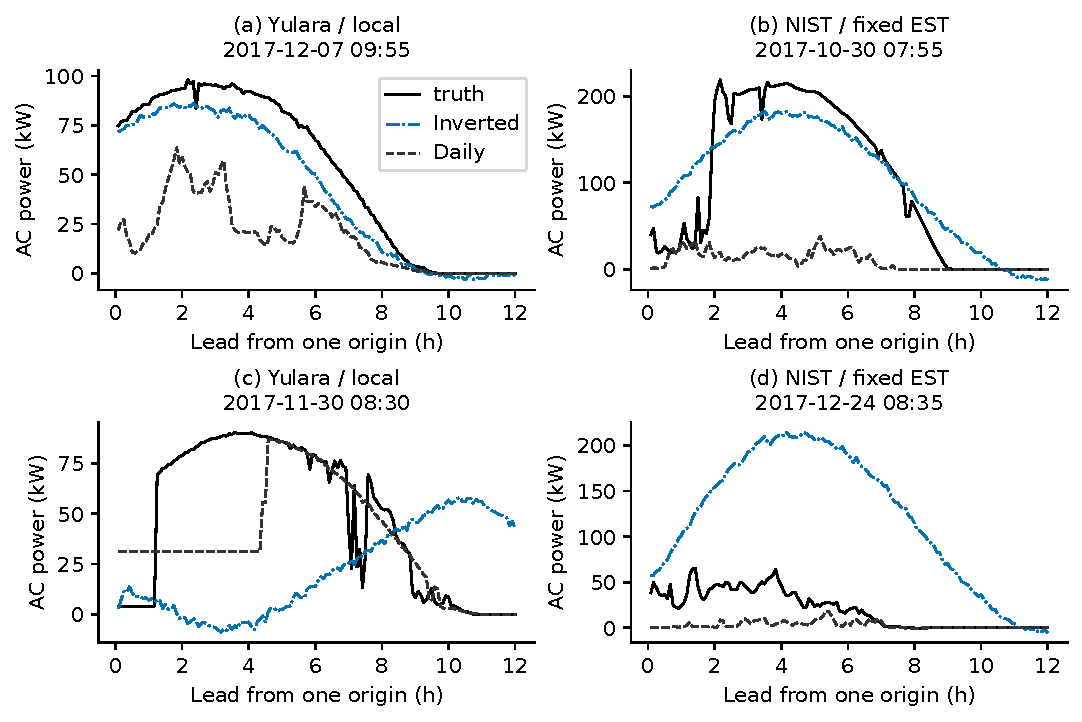
\includegraphics[width=0.98\textwidth,height=0.86\textheight,keepaspectratio]{fixed_period_figures/figS7_cases_extremes.pdf}
\caption{Post hoc diagnostic extremes seed42 trajectories. Fixed cases use the first eligible origin on or after each month’s 15th at 10:00; extremes use original Daily SSE differences and are not representative frequencies.}
\label{figs:figS7_cases_extremes}
\end{figure}
\clearpage\begin{figure}[p]\centering
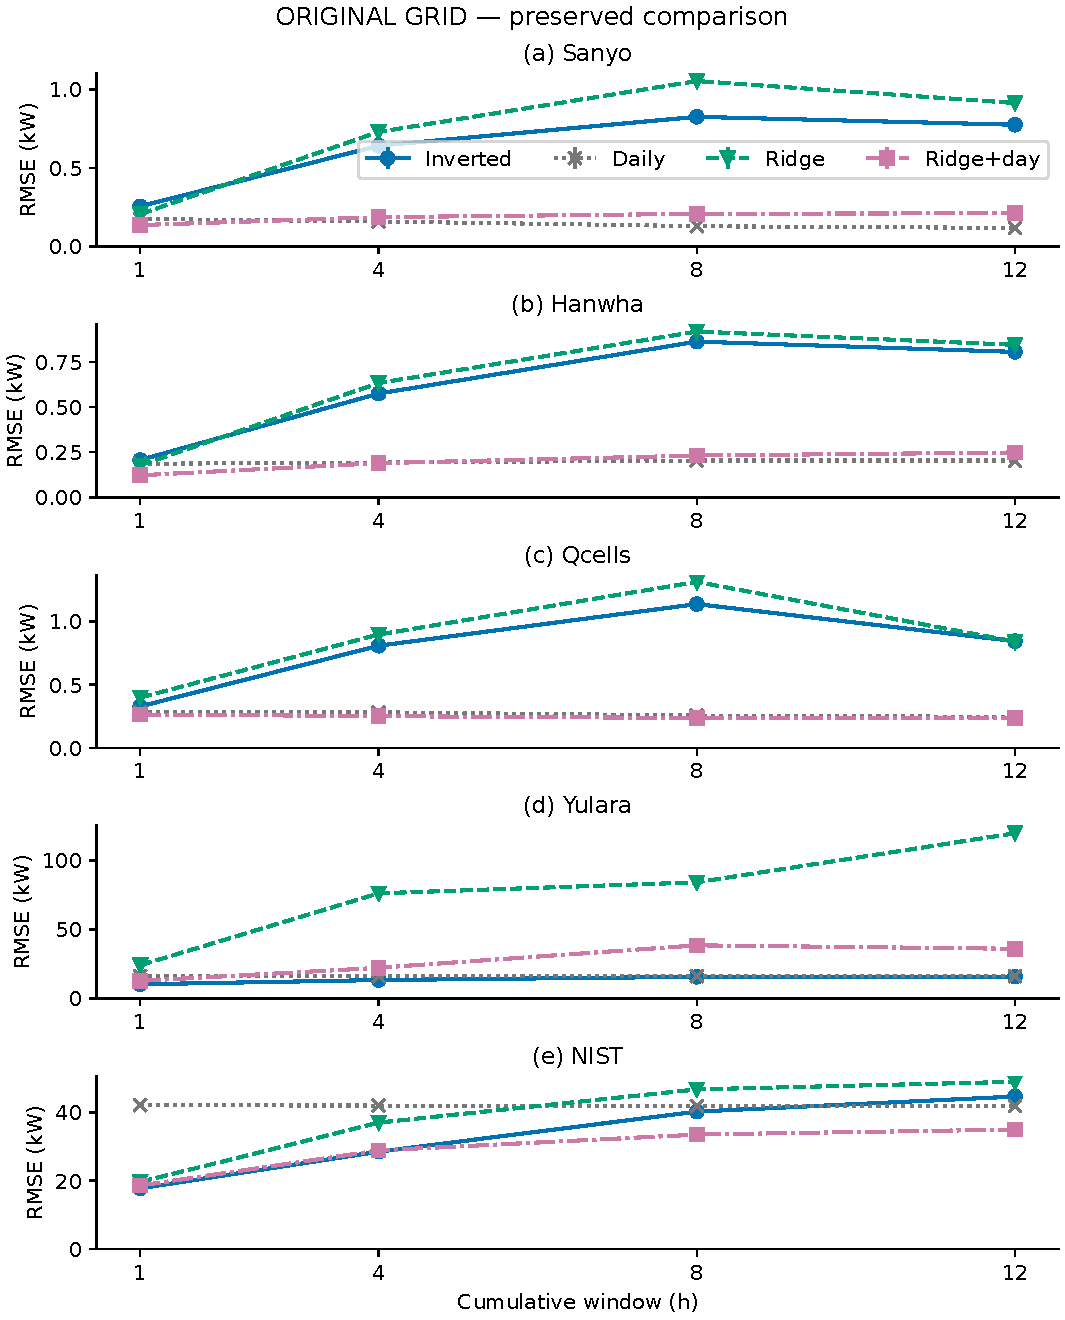
\includegraphics[width=0.98\textwidth,height=0.86\textheight,keepaspectratio]{fixed_period_figures/figS8_ridge.pdf}
\caption{\textbf{Original grid.} Post hoc Ridge with recent history and Ridge plus available previous-day trajectory; alphas selected on Validation only. Daily-matched full targets are identical to the neural comparison. Ridge is deterministic; neural bars are three-seed SD.}
\label{figs:figS8_ridge}
\end{figure}
\clearpage\begin{figure}[p]\centering
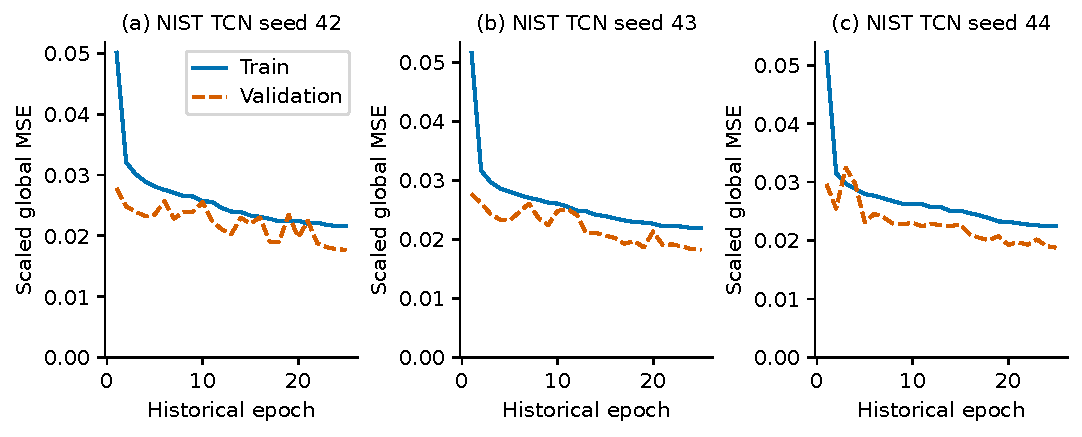
\includegraphics[width=0.98\textwidth,height=0.86\textheight,keepaspectratio]{fixed_period_figures/figS9_learning_budget.pdf}
\caption{Historical NIST TCN learning records. All three selected checkpoints occur at the fixed maximum budget of 25 epochs. These curves document the budget boundary, not convergence or a new fit.}
\label{figs:figS9_learning_budget}
\end{figure}
